\documentclass{beamer}
\usepackage[utf8]{inputenc}
\usepackage[T1]{fontenc}
\usepackage{amsmath, amsthm}
\usepackage{animate} %for gif
\usepackage{graphicx}
\theoremstyle{plain}
\newtheorem{proposition}{Proposition}
\theoremstyle{definition}
\theoremstyle{remark}
\newtheorem{remark}{Remark}
\DeclareMathOperator*{\argmax}{arg\,max}
\DeclareMathOperator*{\argmin}{arg\,min}
\usepackage[
   backend=biber,        
   sorting=nyt,         
   citestyle=authoryear,
   bibstyle=alphabetic, 
]{biblatex}
\addbibresource{references.bib}
\usepackage{listings}
\usepackage{caption}
\usepackage[ruled,vlined]{algorithm2e}
\usepackage{tikz}
\usetikzlibrary{mindmap, trees, calc}
\lstset{basicstyle=\ttfamily\footnotesize,numbers=left}

% Choix du thème Beamer (ex: Madrid)
\usetheme{metropolis}

% Titre et infos
\title{Soft Actor Critic: Off-Policy Maximum Entropy Deep Reinforcement Learning with a Stochastic Actor}
\subtitle{}
\author{Lucien LE GALL}
\date{\today}

\begin{document}

% Page de titre
\begin{frame}
    \centering % Centre tous les éléments
    \vspace{0.2cm} % Ajuste la position verticale du logo
    \vspace{-2cm} % Espacement entre le logo et le titre 
    \titlepage
    Based on the article: \parencite{haarnoja2018softactorcriticoffpolicymaximum}
\end{frame}


\section{Introduction and context}
\begin{frame}{Accurate Recap of the context}
    \centering
    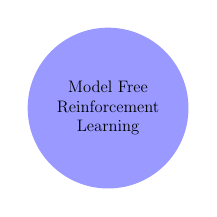
\begin{tikzpicture}[
        mindmap, 
        concept color=blue!40, 
        every node/.style = {
            concept, 
            inner sep=1pt, 
            scale=0.5,
            text width=3cm
        }, 
        every annotation/.append style = {
            fill = red!40,
            text width = 3cm
        },
        scale=0.8]
        \node{Model Free Reinforcement Learning};
    \end{tikzpicture}
\end{frame}

\begin{frame}{Accurate Recap of the context}
    \centering
    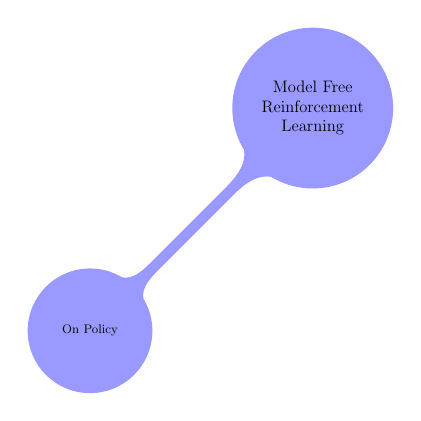
\begin{tikzpicture}[
        mindmap, 
        concept color=blue!40, 
        every node/.style = {
            concept, 
            inner sep=1pt, 
            scale=0.5,
            text width=3cm
        }, 
        every annotation/.append style = {
            fill = red!40,
            text width = 3cm
        },
        scale=0.8]
        \node{Model Free Reinforcement Learning}
            child[grow = south west]{node (2) {On Policy}
            };
    \end{tikzpicture}
\end{frame}

\begin{frame}{Accurate Recap of the context}
    \centering
    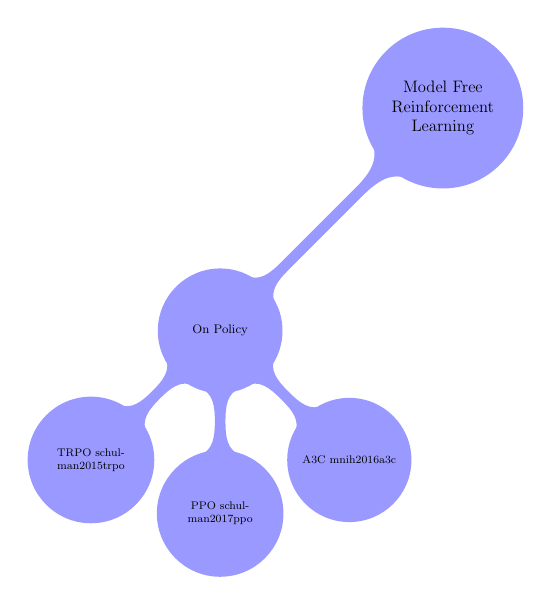
\begin{tikzpicture}[
        mindmap, 
        concept color=blue!40, 
        every node/.style = {
            concept, 
            inner sep=1pt, 
            scale=0.5,
            text width=3cm
        }, 
        every annotation/.append style = {
            fill = red!40,
            text width = 3cm
        },
        scale=0.8]
        \node{Model Free Reinforcement Learning}
            child[grow = south west]{node (2) {On Policy}
                    child[grow = south west] {node {TRPO \parencite{schulman2015trpo}}}
                    child[grow = down] {node{PPO \parencite{schulman2017ppo}}}
                    child[grow = south east] {node{A$3$C \parencite{mnih2016a3c}}}
            };

    \end{tikzpicture}
\end{frame}

\begin{frame}{Accurate Recap of the context}
    \centering
    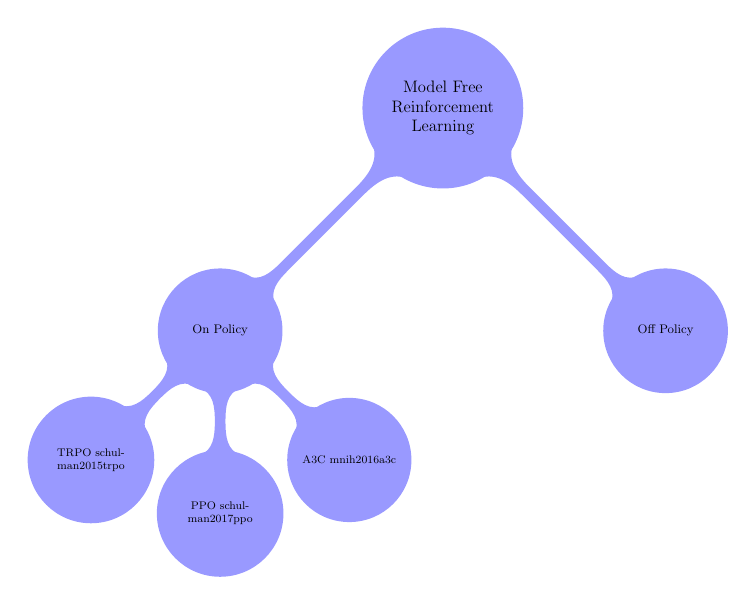
\begin{tikzpicture}[
        mindmap, 
        concept color=blue!40, 
        every node/.style = {
            concept, 
            inner sep=1pt, 
            scale=0.5,
            text width=3cm
        }, 
        every annotation/.append style = {
            fill = red!40,
            text width = 3cm
        },
        scale=0.8]
        \node{Model Free Reinforcement Learning}
            child[grow = south west]{node (2) {On Policy}
                    child[grow = south west] {node {TRPO \parencite{schulman2015trpo}}}
                    child[grow = down] {node{PPO \parencite{schulman2017ppo}}}
                    child[grow = south east] {node{A$3$C \parencite{mnih2016a3c}}}
            }
            child[grow = south east]{node (1) {Off Policy}
            };

    \end{tikzpicture}
\end{frame}

\begin{frame}{Accurate Recap of the context}
    \centering
    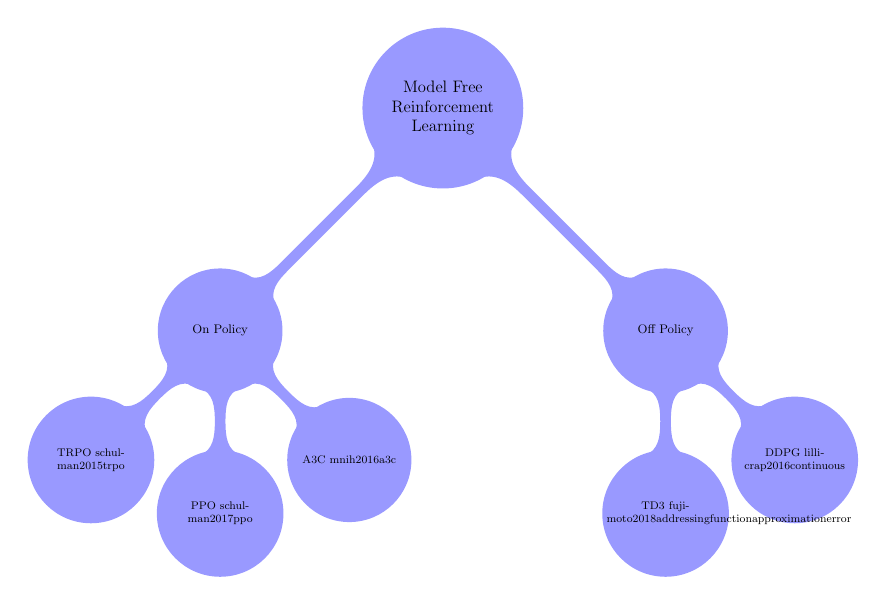
\begin{tikzpicture}[
        mindmap, 
        concept color=blue!40, 
        every node/.style = {
            concept, 
            inner sep=1pt, 
            scale=0.5,
            text width=3cm
        }, 
        every annotation/.append style = {
            fill = red!40,
            text width = 3cm
        },
        scale=0.8]
        \node{Model Free Reinforcement Learning}
            child[grow = south west]{node (2) {On Policy}
                    child[grow = south west] {node {TRPO \parencite{schulman2015trpo}}}
                    child[grow = down] {node{PPO \parencite{schulman2017ppo}}}
                    child[grow = south east] {node{A$3$C \parencite{mnih2016a3c}}}
            }
            child[grow = south east]{node (1) {Off Policy}
                child[grow = south east] {node{DDPG \parencite{lillicrap2016continuous}}}
                child[grow = down] {node {TD3 \parencite{fujimoto2018addressingfunctionapproximationerror}}}
                };

    \end{tikzpicture}
\end{frame}

\begin{frame}{Accurate Recap of the context}
    \centering
    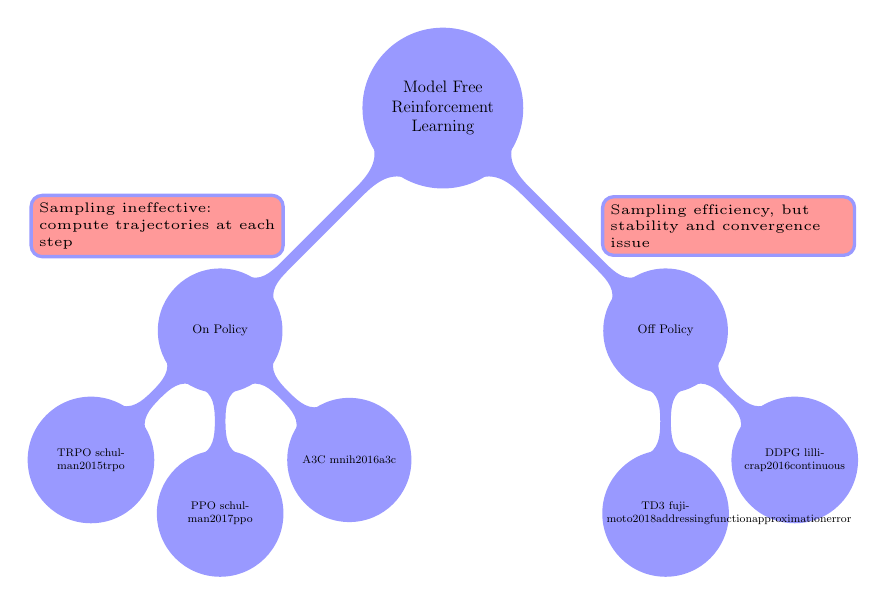
\begin{tikzpicture}[
        mindmap, 
        concept color=blue!40, 
        every node/.style = {
            concept, 
            inner sep=1pt, 
            scale=0.5,
            text width=3cm
        }, 
        every annotation/.append style = {
            fill = red!40,
            text width = 3cm,
            scale=2
        },
        scale=0.8]
        \node{Model Free Reinforcement Learning}
            child[grow = south west]{node (2) {On Policy}
                    child[grow = south west] {node {TRPO \parencite{schulman2015trpo}}}
                    child[grow = down] {node{PPO \parencite{schulman2017ppo}}}
                    child[grow = south east] {node{A$3$C \parencite{mnih2016a3c}}}
            }
            child[grow = south east]{node (1) {Off Policy}
                child[grow = south east] {node{DDPG \parencite{lillicrap2016continuous}}}
                child[grow = down] {node {TD3 \parencite{fujimoto2018addressingfunctionapproximationerror}}}
                };
        \node[annotation] at ($(1.north) + (1,0.7)$)
        {
            Sampling efficiency, but stability and convergence issue
        };
        \node[annotation] at ($(2.north) + (-1,0.7)$)
        {
            Sampling ineffective: compute trajectories at each step
        };
    \end{tikzpicture}
\end{frame}

\section{Soft Policy Iteration}
\begin{frame}{Augmented reward}
The objective function is defined as:
\begin{equation}
    J(\pi)=\displaystyle\sum_{t=0}^{T}\mathbb{E}_{s_t\sim \mu, a_t\sim \pi}(r(s_t,a_t)+\alpha\mathcal{H}(\pi(\cdot|s_t)))
\end{equation}

Where the entropy is the following:

\begin{equation}
    \mathcal{H}(\pi(\cdot|s_t))
    = - \mathbb{E}_{a_t \sim \pi}\big[\log \pi(a_t \mid s_t)\big]
\end{equation}

Introducing a reward \textcolor{blue}{\emph{augmented} reward} \textcolor{blue}{$r_{\pi}(s,a)=r(s,a)+\mathbb{E}_{s'\sim \mu}(\mathcal{H}(\pi(\cdot|s')))$} for all $(s,a)\in \mathcal{S}\times \mathcal{A}$, one can rewrite the objective function as the well-known finite horizon objective function for MDPs: $J(\pi)=\mathbb{E}_{s\sim \mu}(v_{\pi}(s))$.
\end{frame}

\begin{frame}{Soft Policy evaluation: classic policy evaluation but modified reward}
One can derive the policy evaluation presented in the paper using the \textcolor{blue}{Bellman equation \parencite{suttonbarto1998}}.
\begin{align*}
    q(s,a)&=r_{\pi}(s,a)+\gamma\displaystyle\sum_{s'\in \mathcal{S}}p(s'|s,a) v(s')\ \text{(Bellman equation)}\\
    &=r(s,a)-\gamma\displaystyle\sum_{s'\in \mathcal{S}}\sum_{a'\in \mathcal{A}}p(s'|s,a)\pi(a'|s')\log(\pi(a'|s'))\\
    &+\gamma\sum_{s'\in \mathcal{S}}\sum_{a'\in\mathcal{A}}p(s'|s,a) \pi(a'|s')q(s',a')
\end{align*}
One deduces:
\begin{equation}
    q(s,a)=r(s,a)+\gamma\mathbb{E}_{s\sim \mu}(\bar v(s))
    \label{eqn:augmented_bellman_equation}
\end{equation}
with the \textcolor{blue}{\emph{augmented} value function defined} as:
\begin{equation}
    \bar v(s)=\mathbb E_{a\sim \pi}(q(s,a)-\log(\pi(a|s)))
    \label{eqn:augmented_value_function}
\end{equation}

\end{frame}

\begin{frame}{Soft Policy improvement}
The policy improvement step is the following for each state $s\in\mathcal{S}$
\begin{equation}
    \pi_{\text{new}}(a|s)=\displaystyle\argmin_{\pi'\in\Pi}{D_{\text{KL}}\left(\pi'(\cdot|s)\Bigg\|\dfrac{\exp(q^{\pi^{\text{old}}}(s,\cdot))}{Z^{\pi^{\text{old}}}(s)}\right)}
    \label{eqn:soft_policy_improvement}
\end{equation}
Where the Kullback-Leibler divergence ensures a projection of the improve policy over a desired set of policies $\Pi$. One can easily show that:


\begin{proposition}[Soft Policy improvement] If a policy $\pi^{\text{new}}(\cdot|s)$ fulfilled \ref{eqn:soft_policy_improvement}, and $\Pi$ is the set of distribution over $\mathcal{A}$, then:
\begin{equation}
\pi_{\text{new}}(a|s)=\dfrac{\exp(q^{\pi^{\text{old}}}(s,a))}{\displaystyle\sum_{a\in \mathcal{A}}\exp(q^{\pi^{\text{old}}}(s,a))}
\end{equation}
\label{prop:soft_policy_improvement}
\end{proposition}
\begin{proof}
    See in appendix A (page \ref{app:A}).
\end{proof}
\end{frame}

\begin{frame}{Convergence of the algorithm}
The policy evaluation algorithm converges due to two facts: 
\begin{enumerate}
    \item \textcolor{blue}{Contraction of the \emph{soft Bellman operator}} which ensures the convergences of the $q$-function.
    \item \textcolor{blue}{The soft policy improvement} which ensures that we improve the $q$-function at each step.
\end{enumerate}
    
\end{frame}

\begin{frame}{Algorithm}
\footnotesize
\begin{algorithm}[H]
\caption{Soft Policy Iteration}
\label{alg:policy_iteration}
\textbf{Input:} Initialise $q$ and $\pi$\\
\BlankLine
\ForEach{$i$ in $[\![1,N_{\text{iter}}]\!]$}{ 
\textbf{Policy evaluation}\\
    \ForEach{$j$ in $[\![1,N_{q}]\!]$}{
        \ForEach{$s$ in $\mathcal{S}$}{
            \ForEach{$a$ in $\mathcal{A}$}{
                acc $\leftarrow 0$\\
                \ForEach{$s'$ in $\mathcal{S}$}{
                    \ForEach{$a'$ in $\mathcal{A}$}{
                        acc $\leftarrow p(s'|s,a) \pi(a'|s')q(s',a') + p(s'|s,a) \pi(a'|s')\log(\pi(a'|s'))$
                    }
                }
            $q(s,a)\leftarrow r(s,a)+\gamma\times$acc
            }
        }
    }
\textbf{Policy improvement}
$\pi(a|s)\leftarrow\dfrac{\exp(q^{\pi}(s,a))}{\displaystyle\sum_{a\in \mathcal{A}}\exp(q^{\pi}(s,a))}$
}
\end{algorithm}
\end{frame}

\begin{frame}{Numerical results with \lstinline{env = gym.make("Taxi-v3")}}
    \centering
    \animategraphics[
        autoplay,
        loop,
        width=0.9\textwidth
    ]{120}{Captions/Soft_Policy_iteration/Soft_policy_iteration-}{0}{80}\\

\textcolor{blue}{Soft Policy iteration only works with finite states and actions space => need to developp more robust methods for continuous spaces}

\end{frame}

\section{Soft Actor Critic}
\begin{frame}{Soft Actor Critic}
    For continous spaces, one need to introduce specific function approxiators:
    \footnotesize
    \begin{itemize}
        \item Value function:
    \begin{equation}
    J_{\bar v}(\phi)=\mathbb{E}_{s_t\sim\mathcal{D}}\left[\dfrac{1}{2}\left(\bar{v}_{\phi}(s_t)-\underbrace{\mathbb{E}_{a_t\sim\pi_{\phi}}[q_{\theta}(s_t,a_t)-\log(\pi_{\phi}(a_t|s_t))]}_{\text{Approximation of the augmented value function given by \ref{eqn:augmented_value_function}}}\right)^2\right]
    \end{equation}
        \item  $q$ function:
    \begin{equation}
        J_q(\theta)=\mathbb{E}_{(s_t,a_t)\sim\mathcal{D}}\left[\dfrac{1}{2}\left(Q_{\theta}(s_t,a_t)-\underbrace{(r(s_t,a_t)+\gamma\mathbb{E}_{s_{t+1}\sim \mu} [\bar v_{\bar \psi}(s_{t+1})])}_{\text{Approximation of the real $q$ value given by \ref{eqn:augmented_bellman_equation}}}\right)^2\right]
    \end{equation}
        \item $\pi$:
    \begin{equation}
        J_{\pi}(\phi)=\mathbb{E}_{s_t\sim\mathcal{D}}\left[D_{\text{KL}}\left(\pi_{\phi}(\cdot|s_t)\Bigg\|\dfrac{q_{\theta}(s_t,\cdot)}{Z_{\theta}(s_t)}\right)\right]
    \end{equation}
    \end{itemize}
    One can now perform a \textcolor{blue}{stochastic gradient descent}.
\end{frame}

\begin{frame}{Algorithm}
\footnotesize
\begin{algorithm}[H]
    \DontPrintSemicolon
    \SetKwBlock{Init}{Initialize:}{}
    \Init{
        Parameters $\psi, \theta_1, \theta_2, \phi$\;
        Replay buffer $\mathcal{D} \leftarrow \emptyset$\ \tcp*{used for Off-Policy learning}
    }
    
    \For{each iteration}{
        \For{each environment step}{
            $a_t \sim \pi_\phi(a_t|s_t)$ \tcp*{Sample action}
            $s_{t+1} \sim p(s_{t+1}|s_t, a_t)$ \tcp*{Step environment}
            $\mathcal{D} \leftarrow \mathcal{D} \cup \{(s_t, a_t, r_t, s_{t+1})\}$\;
        }
        
        \For{each gradient step}{
            \tcp*{Neural Networks over a batch $B$ selected over $\mathcal{D}$ and compute gradient \textit{via} backpropagation}
            $\psi \leftarrow \psi - \lambda_V\hat{\nabla}_\psi J_V(\psi)$\\
            $\phi \leftarrow \phi - \lambda_\pi \hat{\nabla}_\phi J_\pi(\phi)$ \tcp*{Update Policy}
            $\theta_i \leftarrow \theta_i - \lambda_q \hat{\nabla}_{\theta_i} J_q(\theta_i)$ for $i \in \{1,2\}$ \tcp*{Update q-networks}
            $\bar \psi = \tau \psi +(1-\tau)\bar \psi$
        }
    }
    \caption{Soft Actor-Critic (SAC)}
\end{algorithm}
\end{frame}

\begin{frame}{Pratical implementation of the code}
The code involves several ideas:
\begin{itemize}
    \item Use function approximation to deal with continuous functions.
    \item Two differents Neural Networks for the policy (actor) and the $q$ function (Critic).
    \item Perform Stochastic gradient descent.
    \item Replay buffer to perform off policy learning.
\end{itemize} 
as well as keeping this idea of \textcolor{blue}{entropy} to help for stabilization.
\end{frame}

\begin{frame}{Practical Implementation of the Code}
    \begin{itemize}
        \item \lstinline{next_values = next_q_values - entropy_scale * next_log_pis} and \lstinline{q_targets = rewards + discounts * next_values}
        corresponds respectively to the estimation of the value and of the estimated $\hat q$: $v(s)=\mathbb E_{a\sim \pi}(q(s,a)-\log(\pi(a|s)))$ (\ref{eqn:augmented_value_function}),
        $\hat q(s_t,a_t) = r(s_t,a_t) + \gamma \mathbb{E}_{s_{t+1}\sim p}[v_{\bar\phi}(s_{t+1})]$
        \item \textbf{Update of $\theta$ (Critic):} 
        \lstinline{q_losses = 0.5*(tf.losses.MSE(y_true=q_targets, y_pred=q_values))} 
        corresponds to:
        $J_q(\theta)=\mathbb{E}_{(s_t,a_t)\sim \mathcal D}\left[\dfrac{1}{2}\left(q_\theta(s_t,a_t)-\hat q(s_t,a_t)\right)^2\right]$
        \item \textbf{Update of $\phi$ (Actor):} 
        \lstinline{policy_losses = entropy_scale * log_pis - q_log_targets}
        corresponds to:\\
        $J_\pi(q)=\mathbb{E}_{s_t\sim\mathcal{D}, \epsilon_t\sim\mathcal{N}}[\log \pi_{\phi}(f_{\phi}(\epsilon_t; s_t)|s_t)- q_{\theta}(s_t, f_{\phi}(\epsilon_t; s_t))].$
    \end{itemize}
    In fact, \textcolor{blue}{a gradient descent on $\phi$ is unuseful}.
\end{frame}

\begin{frame}[fragile]{Difficulties Cloning the GitHub Repository}
Creating the SAC environment using
\lstinline{conda env create -f environment.yml}
was impossible for the SAC repository (even for the most recent version), due to outdated dependencies.
That results in the following errors:
\footnotesize
\begin{lstlisting}
Could not solve for environment specs.
The following packages are incompatible:
- joblib ==0.10.3
  - joblib 0.10.3 requires
    - python =3.5 *, which can be installed;
  - joblib 0.10.3 requires
    - python =3.4 *, which does not exist
      (possibly due to a missing channel);
  - joblib 0.10.3 requires
    - python =2.7 *, but no viable options are available:
      - python [2.7.13|2.7.14|...|2.7.18] requires
        - vc =9 *, which can be installed;
      - python 2.7.12 conflicts with all previously
        installable versions...
\end{lstlisting}
\end{frame}

\section{Results and conclusion}
\begin{frame}{Results presented in the article: Comparaison between different algorithms}
    \begin{figure}[H]
        \centering
        \includegraphics[width=\textwidth]{Captions/Results_article/Results.png}
        \caption{Results: Comparaison between different algorithms on the Mujoco environment}
    \end{figure}
\end{frame}

\begin{frame}{Results presented in the article: Stochastic VS deterministic}
    \begin{figure}[H]
        \centering
        \includegraphics[width=0.8\textwidth]{Captions/Results_article/deterministic_stochastic.png}
        \caption{Results: Comparaison between different stochastic policy and deterministic policy for the SAC algorithm}
    \end{figure}
\end{frame}

\begin{frame}{Results presented in the article: Parameters influence}
    \begin{figure}[H]
        \centering
        \includegraphics[width=\textwidth]{Captions/Results_article/parameters.png}
        \caption{Results: Parameters influence of SAC}
    \end{figure}
\end{frame}

\begin{frame}{Our attempt to reproduce the results}
        \begin{figure}[H]
        \centering
        \includegraphics[width=\textwidth]{Captions/Results_personnal/Personnal_result.png}
        \caption{Personnal result implemented with the Stable Baseline3 library}
    \end{figure}
\end{frame}

\begin{frame}{Appendix A: Proof for proposition \ref{prop:soft_policy_improvement}}
    \label{app:A}
We want to compute \ref{eqn:soft_policy_improvement} $\displaystyle\argmin_{\pi'\in\Pi}{D_{\text{KL}}\left(\pi'(\cdot|s)\Bigg\|\dfrac{\exp(q^{\pi^{\text{old}}}(s,\cdot))}{Z^{\pi^{\text{old}}}(s)}\right)}$
 One has:
\begin{align*}
D_{\text{KL}}\Bigg(\pi'(\cdot|s) \Bigg\| \frac{\exp(q^{\pi^{\text{old}}}(s,\cdot))}{Z^{\pi^{\text{old}}}(s)} \Bigg) 
&= \sum_{a\in \mathcal{A}} \pi'(a|s) \log \left( \frac{\pi'(a|s) Z^{\pi^{\text{old}}}(s)}{\exp(q^{\pi^{\text{old}}}(s,a))} \right) \\
&= \sum_{a\in \mathcal{A}} \pi'(a|s) \log \pi'(a|s)\\
&- \sum_{a\in \mathcal{A}} \pi'(a|s) q^{\pi^{\text{old}}}(s,a) + \log Z^{\pi^{\text{old}}}(s)\\
&:=J(\pi'(\cdot|s))
\end{align*}
\end{frame}

\begin{frame}{Appendix A: Proof for proposition \ref{prop:soft_policy_improvement}}
$J$ is a strictly convex and continuous function over the compact set which is the simplex, so it has a unique minimum.  
We consider the Lagrangian function $\mathcal{L}(\pi',\lambda) = J(\pi'(\cdot|s)) + \lambda \left(\displaystyle\sum_{a\in \mathcal{A}} \pi'(a|s) - 1 \right)$

The minimum is reached when the gradient w.r.t.\ $\pi'$ vanishes:
$\frac{\partial \mathcal{L}}{\partial \pi'(a|s)} = \log \pi'(a|s) + 1 - q^{\pi^{\text{old}}}(s,a) + \lambda = 0, \quad \forall a\in\mathcal{A}.$

Taking into account the condition $\displaystyle\sum_{a\in \mathcal{A}} \pi'(a|s)=1$ helps to find $\lambda$ which leads to: $\pi^*(a|s) = \frac{\exp(q^{\pi^{\text{old}}}(s,a))}{\sum_{b\in\mathcal{A}} \exp(q^{\pi^{\text{old}}}(s,b))}$.
\end{frame}

\begin{frame}{Appendix B: TRPO and PPO}
    Using like a Taylor-expansion, one get that:
    \begin{align*}
    V(\pi') &= V(\pi) + (1-\gamma)\, \mathbb{E}_{S \sim d_\pi, \, A \sim \pi} \left[ 
    \frac{\pi'(A|S)}{\pi(A|S)} \, a_\pi(S,A) 
    \right]\\ 
    &+ O\left( \mathbb{E}_{S \sim d_\pi} \left[ D_{\mathrm{KL}}\big(\pi'(\cdot|S) \,\|\, \pi(\cdot|S)\big) \right] \right)
    \end{align*}
    One aims to achieve directly a policy update:
    \begin{equation}
        \begin{aligned}
        \theta_{k+1} &\in \arg\max_\theta 
        L_{\pi_{\theta_k}}(\pi_\theta) 
        \;\; \triangleq \;\;
        \mathbb{E}_{\pi_{\theta_k}} \Bigg[ 
        \sum_{t=0}^{\infty} \gamma^t 
        \frac{\pi_\theta(A_t|S_t)}{\pi_{\theta_k}(A_t|S_t)} 
        a_{\pi_{\theta_k}}(S_t, A_t) 
        \Bigg] \\
        &\text{s.t.} \quad 
        \mathbb{E}_{S \sim d_{\pi_{\theta_k}}} \Big[ 
        D_{\mathrm{KL}}(\pi_\theta(\cdot|S) \,\|\, \pi_{\theta_k}(\cdot|S)) 
        \Big] \le \delta
        \end{aligned}
    \end{equation}
This is the main idea in PPO \parencite{schulman2015trpo}, while in TPO achieves gradient clipping over \parencite{schulman2017ppo}.

\end{frame}

\begin{frame}{Appendix C : DDPG and TD3}
    Let's recap the optimal Bellman equation for the $q$ function.
    \begin{equation}
        q^*(s,a) = \mathbb{E}_{s'\sim \mu}\left[r(s,a)+\gamma\max_{a'}(q^*(s',a'))\right]
    \end{equation}
    From this idea, one can derive a squared Bellman error (MSBE):
    \begin{equation}
   L(\phi, {\mathcal D}) = \underset{(s,a,r,s',d) \sim {\mathcal D}}{{\mathrm E}}\left[
    \Bigg( q_{\phi}(s,a) - \left(r + \gamma (1 - d) \max_{a'} q_{\phi}(s',a') \right) \Bigg)^2
    \right]
    \end{equation}
    The $(d-1)$ is set for computation reasons.
    $\mathcal{D}$ is a replay-buffer which helps to perform \textcolor{blue}{Off-policy learning}.\\
    TD3 is based on this idea but \textcolor{blue}{introduces Double-q Learning to reduce positive bias}.
\end{frame}


\begin{frame}[allowframebreaks] {References}
\printbibliography
\end{frame}

\end{document}